\documentclass{article}
\usepackage{unipr_org_notes}
% grafici
\usepackage{pgfplots}
\usepackage{float}
\usepackage[T1]{fontenc}
\usepackage{lmodern}
\usepackage{tikz}
\usepackage{multirow}

\usetikzlibrary{positioning, arrows.meta}


% colori per abbinare l'immagine
\definecolor{fn_bg}{HTML}{D9EAD3} % Sfondo verde chiaro per 'false negatives'
\definecolor{tn_bg}{HTML}{EFEFEF} % Sfondo grigio chiaro per 'true negatives'
\definecolor{tp_fill}{HTML}{B6D7A8} % Verde più scuro per 'true positives'
\definecolor{fp_fill}{HTML}{F4CCCC} % Rosso chiaro per 'false positives'
\definecolor{datapoint}{HTML}{666666} % Grigio per i punti
\definecolor{fn_area}{HTML}{8A9A83} % Verde/Grigio scuro per area 'relevant' (FN)


\renewcommand{\coursetitle}{Algoritmi per l'intelligenza artificiale}

% \addauthor{Nome}{Mail}


\renewcommand{\authorname}{Simone Colli}
% \renewcommand{\authoremail}{simone.colli@studenti.unipr.it}

\renewcommand{\notedate}{%
    Appunti del corso tenuto dal \textbf{Prof. Vincenzo Bonnici} \\
    \medskip % Aggiunge un piccolo spazio verticale
    Università degli Studi di Parma \\
    Anno Accademico 2025/2026
}


\begin{document}
\maketitle

\tableofcontents

%% blocco slide 1
\section{Introduzione}

Nel campo dell'apprendimento automatico classico,
le attività sono tradizionalmente suddivise in
quattro rami principali:
\begin{itemize}
    \item Apprendimento supervisionato (supervised).
    \item Apprendimento semi-supervisionato (semi-supervised).
    \item Apprendimento non supervisionato (unsupervised).
    \item Apprendimento per rinforzo (reinforcement learning).
\end{itemize}
La distinzione primaria tra queste metodologie di ML risiede nel
livello di disponibilità dei ``dati di verità di base'' (ground truth).
Il \textbf{ground truth} è definito come la conoscenza preliminare dell'output
che il modello dovrebbe produrre per un dato input, basata sull'osservazione
diretta in contrapposizione all'inferenza.

\subsection{Apprendimento automatico supervisionato}

L'apprendimento automatico supervisionato ha come obiettivo l'apprendimento di
una funzione che, dato un \textbf{campione di dati} e i relativi output desiderati,
riesca ad approssimare la funzione sottostante che mappa gli input agli output.
Questa metodologia è comunemente applicata in due principali contesti:
\begin{itemize}
    \item \textbf{Classificazione}: quando si desidera mappare l'input a
    etichette di output discrete.
    \item \textbf{Regressione}: quando l'obiettivo è mappare l'input a un
    output continuo.
\end{itemize}
In entrambi i casi, lo scopo è identificare relazioni o strutture specifiche
nei dati di input che consentano di generare output corretti in modo efficace.
È fondamentale notare che la correttezza dell'output è determinata interamente
dai dati di addestramento, i quali costituiscono la ``verità di base'' che il
modello apprende.

L'efficacia del modello può essere significativamente ridotta dalla
presenza di etichette ``rumorose'' o ``errate'' all'interno dei dati stessi.
Algoritmi notevoli nell'apprendimento supervisionato includono la regressione
logistica, il classificatore bayesiano naif, le macchine a vettori di supporto,
le reti neurali artificiali e le foreste casuali.
Il successo di un modello di ML dipende dalla sua capacità di
generalizzazione. Questo concetto è strettamente connesso alla complessità del
modello, che si riferisce alla complessità della funzione che si sta cercando
di apprendere.
Se si dispone di una quantità limitata di dati o se questi non sono distribuiti
uniformemente, è cruciale optare per un modello a bassa complessità per evitare
situazioni di overfitting.

L'\textbf{overfitting} (sovradattamento) si verifica quando il modello apprende la funzione adattandosi
troppo bene ai soli dati di addestramento, senza cogliere la tendenza o la
struttura effettiva che guida l'output, e quindi non riesce a generalizzare
a nuovi punti dati.
La gestione della generalizzazione è formalizzata tramite il compromesso
\textbf{bias-varianza} (bias-variance tradeoff).
Così facendo il modello presenterà un equilibrio tra:
\begin{itemize}
    \item \textbf{Bias} (distorsione): l'errore sistematico dovuto a ipotesi errate nel
    processo di apprendimento.
    \item \textbf{Varianza}: la quantità in base alla quale l'errore può
    variare tra diversi set di dati.
\end{itemize}
La difficoltà si presenta nel creare un modello che cattura accuratamente le
regolarità dei dati di addestramento e che sia in grado di generalizzare bene
a dati non visti in precedenza.
Generalmente, un aumento del bias (e una conseguente riduzione della
varianza) porta a modelli con livelli di prestazione più stabili e
garantiti, un fattore che può essere cruciale in certe applicazioni.
Per ottenere una buona generalizzazione, la varianza del
modello deve essere attentamente bilanciata in base alla dimensione e
alla complessità dei dati di addestramento.

\begin{nota}{Gestione dei dataset}{}
    Set di dati piccoli e semplici dovrebbero essere gestiti con modelli a
    bassa varianza, mentre set di dati grandi e complessi richiedono
    modelli con una varianza più elevata per poter catturare appieno la
    struttura sottostante dei dati.
\end{nota}

\subsection{Apprendimento automatico semi-supervisionato}

L'apprendimento automatico semi-supervisionato (semi-supervised)
mira a \textbf{etichettare i punti dati senza etichetta}
sfruttando la conoscenza appresa da un piccolo numero di dati già etichettati.
Metodi comuni includono le \textbf{macchine vettoriali di supporto
trasversali} e i \textbf{metodi basati su grafi} (come la
propagazione delle etichette).
\begin{nota}{Vantaggi dell'apprendimento semi-supervisionato}{}
    L'apprendimento semi-supervisionato può migliorare significativamente
    le prestazioni del modello rispetto all'apprendimento supervisionato
    quando si dispone di una quantità limitata di dati etichettati.
    La quantità di dati etichettati limitata si può presentare in
    diversi scenari, come ad esempio:
    \begin{itemize}
        \item Dati etichettati costosi da ottenere (ad esempio, richiedono
        l'intervento umano).
        \item Dati etichettati difficili da ottenere (ad esempio, richiedono
        competenze specialistiche).
        \item Dati etichettati soggetti a vincoli di privacy o etici.
    \end{itemize}
\end{nota}

\begin{esempio}{Rilevamento di messaggi inappropriati}{}
    Nel rilevamento di messaggi inappropriati in un social network,
    è impraticabile etichettare manualmente ogni messaggio.
    Si può, invece, etichettare manualmente un piccolo sottoinsieme
    e usare tecniche semi-supervisionate per comprendere e classificare
    il resto dei contenuti.
\end{esempio}

\subsubsection{Presupposti dell'apprendimento semi-supervisionato}

Per poter giustificare l'utilizzo di pochi dati etichettati per trarre
conclusioni su un grande insieme di dati non etichettati, i metodi
semi-supervisionati si basano su alcuni presupposti fondamentali, quali:
\begin{itemize}
    \item \textbf{Continuità}: Si assume che punti dati ``vicini'' tra
    loro abbiano maggiori probabilità di condividere la stessa
    etichetta.
    \item \textbf{Ipotesi del cluster}: Si presume che i dati formino
    naturalmente dei cluster discreti. Di conseguenza,
    punti nello stesso cluster hanno maggiori probabilità di
    condividere un'etichetta.
    \item \textbf{Presupposto molteplice (manifold)}: Si ipotizza che
    i dati si trovino approssimativamente in uno spazio di
    dimensioni inferiori (un \textit{manifold}) rispetto allo
    spazio di input originale. Questo è rilevante
    quando un sistema con pochi parametri, non osservabile
    direttamente, produce output osservabili ad alta
    dimensione.
\end{itemize}

\subsection{Apprendimento automatico non supervisionato}

L'apprendimento automatico non supervisionato (unsupervised)
opera \textbf{senza output etichettati}. L'obiettivo principale
di questa tecnica è quello di \textbf{dedurre la
struttura naturale} presente all'interno di un insieme di dati,
cercando di trovare \textbf{pattern} intrinseci
nei dati. Le attività più comuni in questo ambito includono:
\begin{itemize}
    \item \textbf{Clustering} (raggruppamento).
    \item \textbf{Apprendimento della rappresentazione}
    (representation learning).
    \item \textbf{Stima della densità} (density estimation).
\end{itemize}
In tutti questi casi, si desidera comprendere la struttura
intrinseca dei dati senza usare etichette fornite
esplicitamente.
Tecniche comuni includono il \textbf{clustering}, l'analisi
dei componenti principali (\textbf{PCA}) e gli \textbf{autocodificatori}
(autoencoders). Le due principali sono il clustering
e la riduzione della dimensionalità dei dati.

\begin{nota}{Valutazione delle prestazioni}{}
Dato che non vengono fornite etichette, nella maggior parte
dei metodi di apprendimento non supervisionato non esiste un
modo specifico per confrontare le prestazioni del modello.
\end{nota}

\subsubsection{Clustering}

Il clustering è una \textbf{tecnica esplorativa} che permette di
aggregare dati in gruppi (detti \textit{cluster}) senza avere
una precedente conoscenza della loro appartenenza a tali
gruppi. Si applica a dataset dove i dati al loro
interno presentano elementi simili tra loro.
All'interno di ogni singolo cluster si troveranno quindi dati
che hanno molte \textbf{caratteristiche simili} tra loro.
È un'ottima tecnica per trovare relazioni tra i dati.

\subsubsection{Riduzione della dimensionalità}

La riduzione della dimensionalità senza supervisione è un
approccio molto usato nella \textbf{pre-elaborazione delle
features}. L'obiettivo principale di questa tecnica è
di \textbf{eliminare il ``rumore''} dai dati.
Un altro utilizzo si trova nella \textbf{rappresentazione dei dati}:
dati in uno spazio delle caratteristiche ad elevata dimensionalità
possono essere proiettati su uno spazio 1D, 2D o 3D per
l'analisi visiva.

\begin{nota}{Compromesso tra riduzione della dimensionalità e prestazioni}{}
    Questa operazione può talvolta causare una minore prestazione predittiva.
    Ma può anche rendere lo spazio dimensionale più compatto, aiutando a
    \textbf{mantenere le informazioni più rilevanti}.
\end{nota}

\subsubsection{Analisi esplorativa}

L'apprendimento non supervisionato è estremamente utile
nell'\textbf{analisi esplorativa dei dati} (exploratory data
analysis), poiché è in grado di \textbf{identificare
automaticamente la struttura} nei dati.
Ad esempio, se un analista volesse segmentare i consumatori,
i metodi di clustering sarebbero un ottimo punto di partenza
per l'analisi.

In situazioni dove è impraticabile o impossibile per un essere
umano proporre tendenze nei dati, l'apprendimento non
supervisionato può fornire \textbf{informazioni iniziali} che
possono poi essere usate per testare o verificare singole
ipotesi.

\subsection{Apprendimento per rinforzo}

L'apprendimento con rinforzo (reinforcement learning) ha l'obiettivo di
realizzare \textbf{agenti autonomi}. Questi agenti devono
essere in grado di scegliere azioni da compiere per conseguire
determinati obiettivi. Questo avviene tramite
l'interazione con l'ambiente in cui sono immersi, con lo scopo
di massimizzare una nozione di \textbf{premio cumulativo}.

%% blocco slide 2
\section{Classificazione}

La classificazione è un'attività dell'apprendimento supervisionato che
consiste nell'assegnare un'etichetta (o classe) a un dato
sulla base di sue caratteristiche osservabili.
Nell'ambito della classificazione si parla di:
\begin{itemize}
    \item \textbf{Feature} (caratteristica): un aspetto direttamente
    osservabile di un fenomeno per il quale si può registrare una
    misura, che sia quantitativa (numerica) o categoriale
    (come vero/falso, rosso/verde, ecc..).
    \item \textbf{Classe}: un concetto astratto
    e generale che ``spiega'' le osservazioni. L'assegnazione
    a una classe costituisce una sintesi delle feature osservate.
    \item \textbf{Label} (etichetta): il nome specifico di una classe.
\end{itemize}

\begin{nota}{Problematica della classificazione}{}

    Alcuni dati possono rendere più complesso l'assegnazione delle classi.
    Questa tipologia di dati è nota come \textbf{outlier statistici}.

\end{nota}

\begin{definizione}{Collezione di dati}{def:collezione_dati}
    Una collezione di dati è un insieme di elementi $P$ di $M$-uple
    del tipo:
    \[
    m_i = (x_{1i}, \ldots, x_{Mi}) \in D_1 \times \ldots \times D_M
    \]
    dove ogni $x_{ji}$ rappresenta una feature ed appartiene ad un possibile
    dominio di valori $D_j$.
    Ogni feature $x_{ji}$ appartiene a un dominio di valori $D_j$.
    I domini possono essere:
    \begin{itemize}
        \item \textbf{Numerici:} (es. $\mathbb{R}$ per valori continui,
        $\mathbb{Z}$ per discreti).
        \item \textbf{Categoriali:} Insiemi finiti di valori (es.
        \{Rosso, Verde, Blu\}).
    \end{itemize}
\end{definizione}

\begin{definizione}{Partizionamento in classi }{def:partizionamento_classi}
Data una collezione di dati \Cref{def:collezione_dati} $P$ e
un insieme finito di $k$ \textbf{etichette} (o classi) $L = \{A_1, \ldots, A_k\}$.

Si dice che $P$ è \textbf{partizionato in classi} se $P$ è suddiviso in
$k$ sottoinsiemi $\{C_1, \ldots, C_k\}$, tali che:
\begin{itemize}
    \item $C_j \subseteq P$, $\forall j \in \{1, \ldots, k\}$
    \item $C_i \cap C_j = \emptyset$, $\forall i \neq j$ (le classi sono
    mutuamente esclusive)
    \item $\bigcup_{j=1}^k C_j = P$ (l'unione delle classi copre l'intero dataset)
\end{itemize}
Ogni sottoinsieme $C_j$ raggruppa tutti e soli gli elementi $m_i \in P$
che sono stati associati all'etichetta (classe) $A_j \in L$.
\end{definizione}

\begin{definizione}{Algoritmo di classificazione}{def:alg_classificazione}
Un \textbf{algoritmo di classificazione} è una funzione computabile
$f: P \mapsto L$, tale che:
\[
f(m \in P) = f(x_1, \ldots, x_m) \in L
\]
Tale funzione $f(m)$ assegna a ogni dato $m$ un'etichetta $A_i$ scelta
tra quelle presenti in $L$ cercando di stimare l'etichetta reale del stesso.

Lo schema di classificazione può produrre due tipi di risultati:
\begin{itemize}
    \item \textbf{Successo} (hit) se l'etichetta stimata $f(m)$
    coincide con l'etichetta reale del dato.
    \item \textbf{Fallimento} (miss) se l'etichetta stimata è errata.
\end{itemize}

\end{definizione}

\begin{nota}{Classificatori \textit{error free}}{}
È generalmente impossibile creare classificatori \textit{error free}.
Per questo motivo è fondamentale fornire stime sul tasso percentuale di
hit/miss.

Il livello tollerabile di errore dipende dalla \textbf{criticità
dell'applicazione}: per applicazioni industriali si può richiedere un
tasso $< 5\%$, mentre per applicazioni mediche un tasso $> 0.5\%$
potrebbe essere già inaccettabile.
\end{nota}

\begin{esempio}{Problema di classificazione: salmoni e branzino}{ex:salmoni_branzino}

Si consideri il problema di distinguere tra salmoni e branzini (sea bass) basandosi
su alcune caratteristiche osservabili.
Le \textbf{feature} utilizzate potrebbero essere la lunghezza, il peso in grammi
e il colore dominante (un attributo qualitativo scelto da un insieme predefinito
come \{blu, grigio, verde\}).
I dati vengono tipicamente organizzati in una tabella, dove ogni riga corrisponde
a un pesce e le colonne ne descrivono le feature.

L'obiettivo è costruire un classificatore che, per ogni nuovo pesce osservato,
sia in grado di riempire la colonna ``specie'' con l'etichetta corretta
(``salmone'' o ``branzino'').
È importante notare che gli errori non hanno lo stesso costo: confondere un
salmone (pesce pregiato) con un branzino (meno pregiato) è un errore più grave
del contrario.

\end{esempio}

\begin{esempio}{Problema di classificazione: studenti e carriera}{ex:studenti_carriera}

Si consideri il problema di predire il futuro successo economico degli studenti
universitari.
Le \textbf{feature} raccolte per ogni studente includono dati anagrafici, il
censo familiare e i voti conseguiti durante la carriera universitaria.
L'obiettivo è costruire un classificatore che predica in quale \textbf{classe}
di reddito si troverà lo studente dieci anni dopo la laurea. Le etichette
(o \textbf{label}) potrebbero essere \{``reddito basso'', ``reddito medio'',
``reddito alto''\}.

È importante notare che, a causa dell'elevato numero di fattori non misurabili
che influenzano la vita di un individuo, una predizione del genere ha un valore
limitato se applicata al singolo studente, che ha un'alta probabilità di essere
classificato erroneamente.

Tuttavia, questo tipo di analisi è estremamente utile a livello statistico e
aggregato, per comprendere le tendenze generali di un'intera popolazione
studentesca e informare politiche educative o economiche.

\end{esempio}

\subsection{Costruire un classificatore}

Il processo di costruzione di un classificatore automatico simula
il fenomeno dell'apprendimento umano o animale, noto come
\textbf{training} (addestramento). L'idea è \textbf{dedurre regole
generali}, applicabili a record non ancora classificati,
partendo dall'osservazione di esempi già noti e ben classificati.

Gli algoritmi e le tecniche di classificazione automatica sono
numerosissimi. Tutti i metodi noti condividono uno \textbf{schema
generale} (Figura \ref{fig:th_02_01}) ben testato e riconosciuto dalla comunità scientifica.

\begin{figure}[H]
    \centering
    \includegraphics[width=0.6\textwidth]{images/th_02/01.png}
    \caption{Schema generale di un sistema di classificazione}
    \label{fig:th_02_01}
\end{figure}

\begin{definizione}{Universo delle osservazioni}{def:universo_osservazioni}
    Si definisce \textbf{universo delle osservazioni} l'insieme
    complessivo dei record (passati, presenti e futuri) relativi ad un fenomeno.
    Molti algoritmi iniziano esaminando un sottoinsieme di questo
    universo, già classificato e ben compreso.
\end{definizione}

Un universo delle osservazioni \Cref{def:universo_osservazioni} 
che rappresenta l'insieme di ``allenamento'', chiamato \textbf{Training Set
(TS)}, è il deposito di informazioni iniziali da cui l'algoritmo
ricava le ``regole'' di classificazione. Le regole ricavate saranno di vario
tipo: statistiche, probabilistiche, fuzzy, funzioni discendenti, ecc.

\subsection{Proprietà di un classificatore}

Un buon insieme di regole di classificazione deve avere tre
importanti proprietà:
\begin{itemize}
    \item \textbf{Semplicità}: Le regole non devono essere troppo
    complicate, per garantire efficienza e basso costo computazionale
    in fase di classificazione.
    \item \textbf{Correttezza sul TS}: Le regole devono essere
    statisticamente sufficientemente corrette quando applicate
    al medesimo Training Set che le ha generate.
    \item \textbf{Generalizzabilità}: Le regole devono essere
    statisticamente corrette anche quando applicate al resto
    dei record dell'universo (dati nuovi, non visti).
\end{itemize}

\begin{nota}{}{}
Il termine \textbf{statisticamente corretto} su un training set indica che il
tasso dei miss non deve superare certe soglie di tolleranza che dipendono
dalla criticità delle applicazioni.
\end{nota}

\subsection{Il problema dell'overfitting}

Le proprietà di correttezza sul TS e di generalizzabilità sono
spesso in conflitto tra loro.
Questo paradosso è noto come \textbf{overfitting} (sovradattamento).
L'overfitting si verifica quando un modello si adatta
``troppo bene'' ai dati del Training Set. Un modello molto
complesso può imparare a memoria le peculiarità e persino
il rumore casuale presente nel TS, ottenendo una correttezza
perfetta su di esso.
Tuttavia, tale modello non avrà appreso la ``tendenza'' generale
dei dati e fallirà nel generalizzare a nuovi record,
poiché la frontiera di decisione che ha appreso è
eccessivamente complessa e specifica per il campione di training.

L'obiettivo non è minimizzare l'errore sul TS (che
porterebbe a un modello complesso e in overfitting), ma
trovare un equilibrio: un modello (es. una retta o una
curva semplice) che, pur commettendo qualche errore sul TS,
catturi la struttura di fondo dei dati e possa quindi
generalizzare meglio.

\subsection{Validazione}

Per ``convalidare'' la proprietà di generalizzazione di un
insieme di regole, si utilizza un metodo che prevede, oltre
al TS, un altro insieme di record già etichettati, detto
\textbf{Control Set (CS)} o \textbf{Test Set}.
Il CS \textbf{non} viene utilizzato durante la fase di
training (cioè per la sintesi delle regole). Viene usato
solo dopo che le regole sono state definite.
Se le regole mostrano sul CS un tasso di errore (miss)
simile a quello ottenuto sul TS, allora si ritiene
che le regole siano \textbf{generalizzabili}.

Poiché anche il CS è un campione casuale, per una stima
più precisa è buona norma ripetere i test con diversi CS,
spesso creati tramite strategie di randomizzazione
nella selezione del TS e del CS dall'universo disponibile.

\subsection{Gestione delle feature e del rumore}

Nella costruzione di un classificatore è cruciale gestire
sia la selezione delle feature che la presenza di rumore.

\subsubsection{Selezione delle feature}
Spesso si rilevano molte feature, ma non tutte sono utili;
alcune possono essere sovrabbondanti o addirittura dannose.
Combinare più feature (es. lunghezza e luminosità dei pesci)
è spesso una strategia conveniente, ma non è detto che
sia sempre la migliore.
L'inclusione di troppe feature, specialmente se irrilevanti,
può amplificare il \"rumore\" e confondere il classificatore.
Una buona pratica è scegliere feature che siano
\textbf{invarianti} alle trasformazioni tipiche della
situazione sperimentale (es. il peso di un pesce è
invariante alle condizioni di luce, la luminanza no).
Inoltre, deve esistere una probabile relazione tra le
feature misurate e la classe da predire.

\subsubsection{Rumore e outlier}
I dati del mondo reale contengono inevitabilmente
\textbf{rumore}, ovvero perturbazioni dovute a fenomeni
non controllabili o non noti. Le cause di tale
spostamento dai valori ``ideali'' possono essere:
\begin{itemize}
    \item \textbf{Endogene}: Interne al fenomeno (es. un pesce
    con una dieta o storia anomala).
    \item \textbf{Esogene}: Dovute all'osservatore o allo
    strumento utilizzato (es. macchina fotografica starata,
    etichettatore distratto).
\end{itemize}

I dati molto ``fuori norma'' rispetto ai valori tipici di una
classe sono definiti \textbf{outlier}.
Un buon algoritmo di classificazione deve essere
\textbf{robusto}, ovvero deve avere una forma di
``protezione'' o resistenza alle deviazioni che il rumore
impone al processo decisionale.

\subsection{Valutazione degli errori}

Contare gli errori è essenziale, ma una singola percentuale
di errore non è sufficientemente descrittiva. Questo perché
non tutti gli errori sono uguali: i \textbf{costi degli errori}
spesso \textbf{non sono uniformi} o simmetrici.

Ad esempio, in una diagnosi medica:
\begin{itemize}
    \item Classificare un sano come malato (Falso Positivo)
    è un errore con un costo relativamente basso (paura, un
    test aggiuntivo).
    \item Classificare un malato come sano (Falso Negativo)
    è un errore gravissimo, che ritarda la diagnosi e
    può costare la vita al paziente.
\end{itemize}

Per analizzare questa asimmetria si usa la
\textbf{matrice di confusione}. È una griglia quadrata
che riporta quante istanze della classe ``reale'' (sulle colonne)
sono state assegnate alla classe ``prevista'' (sulle righe).

\begin{nota}{Matrice di confusione ideale}{}
    Un classificatore perfetto ha come matrice di confusione la
    matrice identica (tutti i valori sulla diagonale principale,
    zero altrove). Un buon classificatore avrà valori
    percentuali bassi al di fuori della diagonale principale.

\end{nota}
\subsection{Fasi di un sistema di classificazione}

Il processo di classificazione automatica si articola in
diverse fasi:
\begin{enumerate}
    \item \textbf{Sensing (o sampling)}: Raccolta dei dati dal
    mondo fisico e loro digitalizzazione.
    \item \textbf{Segmentazione}: Partizione dei dati in unità
    significative, pulizia ed eliminazione di dati irrilevanti.
    \item \textbf{Estrazione delle feature}: Misurazione delle
    caratteristiche (quantitative o qualitative). È cruciale
    scegliere feature invarianti e rilevanti.
    \item \textbf{Classificazione}: Esecuzione dell'algoritmo
    scelto per l'assegnazione delle etichette.
    \item \textbf{Post-processing}: Valutazione della qualità
    della classificazione e dei costi associati agli errori.
    \item \textbf{Decisione}: Utilizzo effettivo del
    classificatore per risolvere il problema reale.
\end{enumerate}

La costruzione di un classificatore è un \textbf{ciclo
iterativo} che prevede la raccolta dei dati, la selezione
delle feature, la scelta di un modello matematico, il
training dell'algoritmo e infine la sua valutazione,
ripetendo i passi per migliorare le prestazioni.
%% blocco slide 3


\section{Tecniche di validazione per la classificazione}

Dopo aver costruito un modello di classificazione, è fondamentale valutarne le
performance. A differenza della regressione, dove si cerca di predire un
valore numerico di output dato uno o più valori di input, nella
classificazione si vuole predire la classe di un oggetto dato uno o più
dati di input di qualsiasi tipo (numerici, categorici, testuali, ecc.).

Per questo motivo gli strumenti che si possono applicare per valutare un modello di
classificazione sono sostanzialmente diversi rispetto alle metriche utilizzate
per valutare i modelli di regressione.

\subsection{Modello di validazione base: Training e Test Set}

L'approccio base per la validazione consiste nel dividere, secondo una certa
\textbf{percentuale} i dati disponibili in due insiemi:

\begin{itemize}
    \item \textbf{Training set (TS)}: Utilizzato per addestrare il
    classificatore. Le etichette (label) di questi dati sono usate per
    addestrare il classificatore.
    \item \textbf{Test set}: Utilizzato per valutare la bontà del modello.
    Le etichette di questo set vengono usate solo per verificare se
    il classificatore ha predetto correttamente.
\end{itemize}

L'obiettivo della validazione non è solo misurare l'errore, ma ha lo scopo di
rispondere a domande più complesse, come:
\begin{itemize}
    \item Il classificatore performa in modo bilanciato su tutte le classi?
    \item Ha delle preferenze?
    \item Tali preferenze da cosa dipendono?
\end{itemize}
Per questo motivo per la valutazione dei classificatori si utilizzano indici
matematici che permettono sia di avere stime oggettive delle performance, sia
di automatizzare anche altre fasi del processo della progettazione o sviluppo
del classificatore.

Gli indici principali relativamente all'aspetto computazionale utilizzati
per valutare un classificatore sono:
\begin{itemize}
    \item \textbf{Accuratezza}: La bontà nel predire correttamente le
    etichette.
    \item \textbf{Robustezza}: La capacità di gestire dati con rumore o valori
    mancanti.
    \item \textbf{Velocità}: Include sia il tempo per costruire il modello
    (training time) sia il tempo per usarlo (classification/prediction time).
    \item \textbf{Scalabilità}: L'efficienza del modello su grandi dataset,
    specialmente se in memoria secondaria.
    \item \textbf{Interpretabilità}: La facilità con cui i risultati del
    modello possono essere compresi.
\end{itemize}

\subsection{Metriche di valutazione}
Per definire le metriche più comuni, si assume un problema di classificazione
binaria. Si assume che l'insieme delle classi $\mathbb{C}$ dell'esperimento
sia composto da due classi: $\mathbb{C}=\{A,B\}$.

Relativamente ad una delle classi è possibile definire alcune misure per
calcolare la bontà dell'algoritmo in valutare tale classe.

Data una classe di interesse (es. A, la classe ``positiva''),
i risultati della classificazione sul test set vengono divisi in quattro
categorie:

\begin{itemize}
    \item True positive (TP).
    \item True negative (TN).
    \item False positive (FP).
    \item False negative (FN).
\end{itemize}

\begin{center}
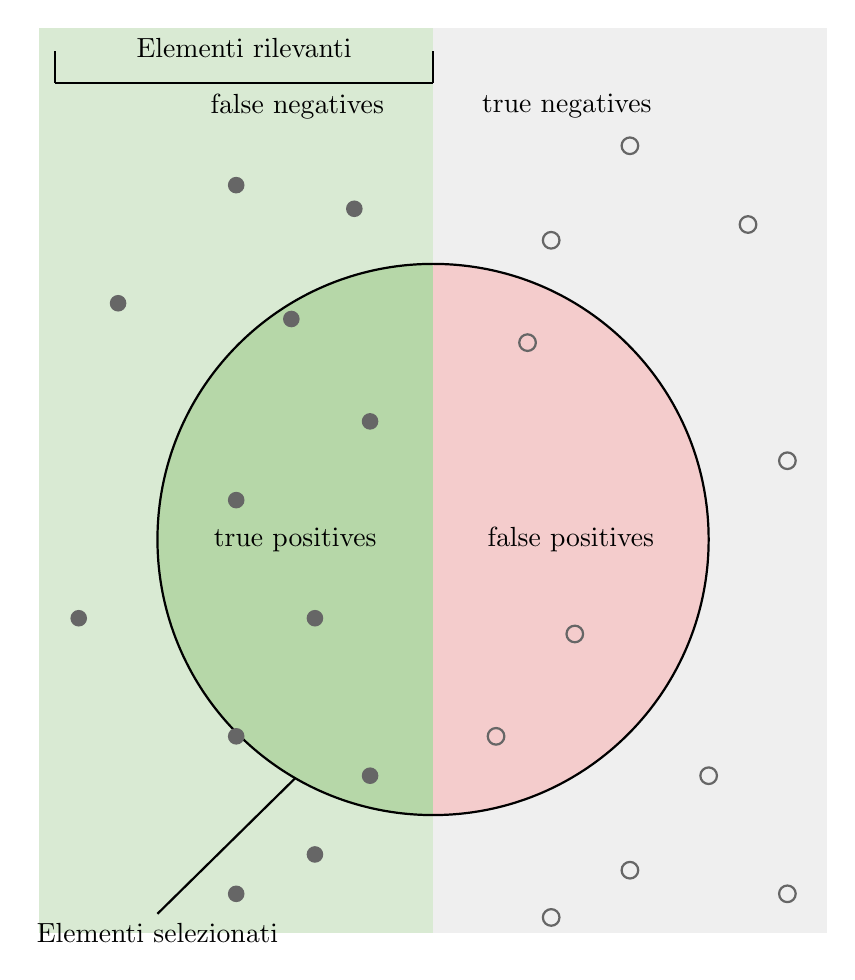
\begin{tikzpicture}[
    % Definiamo stili per i punti dati
    solid_point/.style = {
        circle, 
        fill=datapoint, 
        minimum size=6pt, 
        inner sep=0
    },
    hollow_point/.style = {
        circle, 
        draw=datapoint, 
        thick, 
        minimum size=6pt, 
        inner sep=0
    }
]

% 1. Disegnare le aree di sfondo (Actual)
% Sfondo per\"Relevant\"(Sinistra)
\fill[fn_bg] (-5, -5) rectangle (0, 6.5);
% Sfondo per\"Not Relevant\"(Destra)
\fill[tn_bg] (0, -5) rectangle (5, 6.5);

% 2. Disegnare il cerchio (Selected) e riempirlo
% Riempiamo la metà sinistra (True Positives)
\fill[tp_fill] (90:3.5) arc (90:270:3.5) -- cycle;
% Riempiamo la metà destra (False Positives)
\fill[fp_fill] (90:3.5) arc (90:-90:3.5) -- cycle;

% Disegniamo il bordo nero del cerchio
\draw[thick] (0, 0) circle (3.5cm);

% 3. Posizionare i punti dati
% False Negatives (Solidi, Sinistra, Fuori)
\node[solid_point] at (-2.5, 4.5) {};
\node[solid_point] at (-1, 4.2) {};
\node[solid_point] at (-4, 3) {};
\node[solid_point] at (-4.5, -1) {};
\node[solid_point] at (-2.5, -4.5) {};
\node[solid_point] at (-1.5, -4) {};

% True Positives (Solidi, Sinistra, Dentro)
\node[solid_point] at (-1.8, 2.8) {};
\node[solid_point] at (-0.8, 1.5) {};
\node[solid_point] at (-2.5, 0.5) {};
\node[solid_point] at (-1.5, -1) {};
\node[solid_point] at (-2.5, -2.5) {};
\node[solid_point] at (-0.8, -3) {};

% False Positives (Vuoti, Destra, Dentro)
\node[hollow_point] at (1.2, 2.5) {};
\node[hollow_point] at (1.8, -1.2) {};
\node[hollow_point] at (0.8, -2.5) {};

% True Negatives (Vuoti, Destra, Fuori)
\node[hollow_point] at (2.5, 5) {};
\node[hollow_point] at (4, 4) {};
\node[hollow_point] at (1.5, 3.8) {};
\node[hollow_point] at (4.5, 1) {};
\node[hollow_point] at (3.5, -3) {};
\node[hollow_point] at (2.5, -4.2) {};
\node[hollow_point] at (1.5, -4.8) {};
\node[hollow_point] at (4.5, -4.5) {};

% 4. Aggiungere le etichette
% Etichette di sfondo
\node[anchor=west] at (0.5, 5.5) {true negatives};
\node[anchor=east] at (-0.5, 5.5) {false negatives};

% Etichette del cerchio
\node at (-1.75, 0) {true positives};
\node at (1.75, 0) {false positives};

% Etichetta\"relevant elements\"con la staffa
\draw [thick] (-4.8, 6.2) -- (-4.8, 5.8);
\draw [thick] (-4.8, 5.8) -- (0, 5.8);
\draw [thick] (0, 5.8) -- (0, 6.2);
\node at (-2.4, 5.8) [above=2mm] {Elementi rilevanti};

% Etichetta\"selected elements\"con il puntatore
\node (label_sel) at (-3.5, -5) {Elementi selezionati};
% Il punto sul cerchio è a 240 gradi, raggio 3.5
\draw [thick, -] (label_sel.north) -- (240:3.5);

\end{tikzpicture}
\end{center}

\begin{definizione}{TP, TN, FP, FN}{}

Sia $c: CS \mapsto \mathbb{C}$ la funzione che mappa ogni record $x \in CS$
nella sua classe reale e sia $\tilde{c}: CS \mapsto \mathbb{C}$ il
classificatore che assegna una classe ad $A$.

Sia $C = \{A, B\}$ l'insieme delle classi, composto dalle classi $A$ e $B$.
Prendendo come riferimento la classe $A$ è possibile dividere $CS$ in 4 insiemi:

\begin{itemize}
    \item \textbf{True positive (TP)}: I record $x \in CS$ classificati \textbf{correttamente},
    ovvero la cui classe reale è $A$, quindi $\tilde{c}(x) = c(x) = A$
    \item \textbf{True negative (TN)}: I record $x \in CS$ classificati \textbf{correttamente},
    ovvero la cui classe reale è $B$, quindi $\tilde{c}(x) = c(x) = B$
    \item \textbf{False positive (FP)}: I record $x \in CS$ classificati \textbf{erroneamente},
    ovvero la cui classe reale è $B$, quindi $\tilde{c}(x) = B \ne A = c(x)$
    \item \textbf{False negative (FN)}: I record $x \in CS$ classificati \textbf{erroneamente},
    ovvero la cui classe reale è $B$, quindi $\tilde{c}(x) = A \ne B = c(x)$
\end{itemize}
\end{definizione}

\bigskip
Basandosi su queste quattro categorie, è possibile definire le metriche di
performance più utilizzate.

\begin{definizione}{Precision}{}
Sia $C = \{A, B\}$ l'insieme delle classi, composto dalle classi $A$ e $B$.
La precision (precisione) è la frazione di elementi rilevanti per una classe
di riferimento, $A$, tra tutti gli elementi che il classificatore ha
identificato come $A$.
La precision misura quanto è ``affidabile'' la predizione positiva,
ed è definita come:
\[
Precision = \frac{TP}{TP+FP}
\]

\end{definizione}

\begin{definizione}{Recall}{}
Sia $C = \{A, B\}$ l'insieme delle classi, composto dalle classi $A$ e $B$.
La recall (richiamo o sensitività) è la frazione di elementi rilevanti
(classi A) che sono stati correttamente classificati come A.
Misura la capacità del classificatore di ``trovare'' tutti i positivi.
\[
Recall = \frac{TP}{TP+FN}
\]
\end{definizione}

\begin{center}
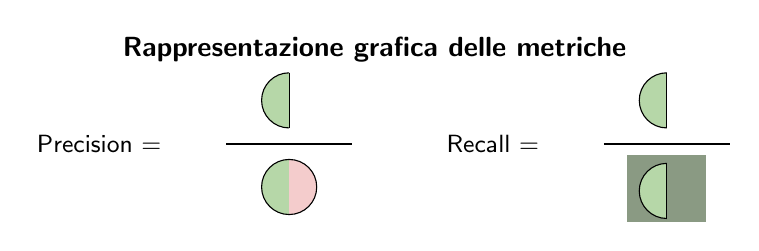
\begin{tikzpicture}[
    font=\sffamily\small,
    radius=0.35cm % Raggio ridotto per i cerchi
]

% --- Titolo ---
\node[font=\sffamily\bfseries] at (3.5, 1.2) {Rappresentazione grafica delle metriche};


% --- Definiamo una forma riutilizzabile per il semicerchio TP ---
\def\tpsemicircle{
    % Arrotondamento verde
    \fill[tp_fill] (90:0.35) arc (90:270:0.35) -- cycle;
    % Bordo dell'arco
    \draw[black] (90:0.35) arc (90:270:0.35);
    % Linea dritta
    \draw[black] (90:0.35) -- (270:0.35);
}

% --- 1. Precision ---
% Etichetta
\node (prec_label) at (0, 0) {Precision =};

% Posizioniamo la frazione a destra dell'etichetta
\begin{scope}[shift={(prec_label.east)}, xshift=1.5cm]
    
    % Numeratore (TP Semicerchio)
    \begin{scope}[yshift=0.55cm]
        \tpsemicircle
    \end{scope}
    
    % Linea di frazione
    \draw[thick] (-0.8, 0) -- (0.8, 0);
    
    % Denominatore (TP + FP Cerchio intero, "selected elements")
    \begin{scope}[yshift=-0.55cm]
        \fill[tp_fill] (90:0.35) arc (90:270:0.35) -- cycle;
        \fill[fp_fill] (90:0.35) arc (90:-90:0.35) -- cycle;
        \draw[black] (0,0) circle (0.35);
    \end{scope}
\end{scope}

% --- 2. Recall ---
% Etichetta
\node (rec_label) at (5, 0) {Recall =};

% Posizioniamo la frazione a destra dell'etichetta
\begin{scope}[shift={(rec_label.east)}, xshift=1.5cm]
    
    % Numeratore (TP Semicerchio)
    \begin{scope}[yshift=0.55cm]
        \tpsemicircle
    \end{scope}
    
    % Linea di frazione
    \draw[thick] (-0.8, 0) -- (0.8, 0);
    
    % Denominatore (Come da tua immagine: Rettangolo scuro [FN] che contiene TP)
    % Questo rappresenta (TP) / (TP + FN) o "relevant elements"
    \begin{scope}[yshift=-0.85cm]
        % Rettangolo scuro di sfondo (FN)
        \fill[fn_area] (-0.5, -0.15) rectangle (0.5, 0.7);
        % Semicerchio TP sovrapposto
        \begin{scope}[yshift=0.25cm]
            \tpsemicircle
        \end{scope}
    \end{scope}
\end{scope}

\end{tikzpicture}
\end{center}

\begin{nota}{Valori ottenuti}{}
Valori alti per entrambe le metriche indicano un buon classificatore.
Spesso, però, si preferisce utilizzare un indice unico che le combini.
\end{nota}
\bigskip
\begin{definizione}{$F_1$-Score}{}
Il $F_1$-Score rappresenta la media armonica di precision e recall.
Fornisce un equilibrio tra le due metriche.
\[
F_{1} = 2 \cdot \frac{Precision \cdot Recall}{Precision + Recall}
      = \frac{2 \cdot TP}{2 \cdot TP + FP + FN}
\]
Come precision e recall, anche l'$F_1$-Score ha un valore compreso tra 0 e 1.
Maggiore è il valore, maggiore è la bontà del classificatore.
\end{definizione}

\begin{nota}{Overfitting}{}
Sebbene un $F_1$-Score alto sia desiderabile, valori molto prossimi a 1
possono essere un campanello d'allarme per l'overfitting.
\end{nota}

\subsection{Accuracy}

\begin{definizione}{Accuracy}{}
La accuracy (accuratezza) misura la quantità totale di oggetti classificati
correttamente (sia positivi che negativi) rispetto al totale degli oggetti.
\[
Accuracy = \frac{TP+TN}{TP+TN+FP+FN}
\]
\end{definizione}

\begin{nota}{Accuratezza per dataset sbilanciati}{}
L'accuracy standard è poco indicata se le classi non sono bilanciate.
Ad esempio, in un dataset con 95 campioni negativi e 5 positivi,
un classificatore ``pigro'' che predice sempre ``negativo'' otterrebbe un'accuratezza
del 95\%, pur essendo totalmente inutile nel riconoscere i positivi.
\end{nota}

In situazione di sbilanciamento delle classi, si preferisce la Balanced accuracy.

\begin{definizione}{Balanced accuracy}{}
La Balanced accuracy (accuratezza bilanciata) è la media tra la sensitività
(per i positivi) e la specificità (per i negativi).
\[
Balanced\ accuracy = \frac{TPR + TNR}{2}
\]
dove:
\begin{itemize}
    \item \textbf{TPR (True Positive Rate)}: È la Recall/Sensitività:
    $TPR = \frac{TP}{TP+FN}$.
    \item \textbf{TNR (True Negative Rate)}: È la Specificità:
    $TNR = \frac{TN}{TN+FP}$.
\end{itemize}
\end{definizione}

\subsection{Altri indici e matrice di confusione}

\begin{definizione}{False Discovery Rate (FDR)}{}
Misura il tasso di errori di tipo I (``false scoperte'' o Falsi positivi)
rispetto a tutte le predizioni positive.
\[
FDR = \frac{FP}{FP+TP} = 1 - Precision
\]
\end{definizione}

\subsubsection{Matrice di confusione}
La matrice di confusione è una tabella che riassume le performance di un
classificatore binario, incrociando le classi reali con quelle predette e
mostrando i conteggi di TP, TN, FP e FN.
È fondamentale perché non tutti gli errori hanno lo stesso costo, come
discusso in precedenza (es. diagnosi medica errata).

\begin{figure}[H]
    \centering
    \includegraphics[width=0.6\textwidth]{images/th_03/01.png}
    \caption{Esempio di matrice di confusione per classificazione binaria.}
\end{figure}

È importante notare che metriche come sensitività, precisione e specificità
dipendono dalla classe presa in considerazione, mentre l'accuratezza è un
indice globale.

\subsection{Area Under the Curve (AUC) e curva ROC}

L'AUC (Area Under the Curve) è una misura basata sulla curva ROC (Receiver
Operating Characteristics).

\begin{definizione}{Curva ROC}{}
Una curva ROC è un grafico che mostra le performance di un classificatore
al variare di un suo parametro (es. una soglia). Mette in relazione il
\textbf{True Positive Rate (TPR)} (sull'asse Y) con il \textbf{False Positive
Rate (FPR)} (sull'asse X).

( $FPR = 1 - Specificit\grave{a} = \frac{FP}{FP+TN}$ ).

Le curve ROC passano sempre per i punti $(0,0)$ e $(1,1)$. Esistono inoltre due
condizioni limite che rappresentano due curve di riferimento:

\begin{itemize}
    \item Una retta che taglia il grafico a 45 gradi passando per l'origine.
    Questa retta rappresenta il caso del \textbf{classificatore casuale} e
    l'area sottesa (AUC) è pari a $0.5$.
    \item Una curva rappresentata dal segmento che dall'origine sale
    verticalmente al punto $(0,1)$ e dal segmento che congiunge il punto
    $(0,1)$ a $(1,1)$. Questa curva ha un'area sottesa di valore pari a 1 e
    rappresenta il \textbf{classificatore perfetto}.
\end{itemize}
\end{definizione}


L'AUC, ha un valore compreso tra 0 e 1, e misura l'intera area bidimensionale
sotto la curva ROC.
\begin{itemize}
    \item \textbf{AUC = 1}: Rappresenta il classificatore perfetto, che
    passa per il punto (0,1)
    \item \textbf{AUC = 0.5}: Rappresenta il classificatore casuale
    (la linea diagonale).
    \item \textbf{AUC = 0}: Rappresenta il classificatore
    ``perfettamente sbagliato'' (che inverte tutte le predizioni).
\end{itemize}
Il valore di AUC (tra 0 e 1) può essere interpretato come la probabilità
che il classificatore assegni un punteggio più alto a un individuo positivo
scelto a caso, rispetto a un individuo negativo scelto a caso.

\subsection{Classificazione multi-classe}

Le misure viste finora (Precision, Recall, $F_1$-score) sono definite per la
classificazione binaria. Per applicarle a problemi con $K > 2$ classi, si
perde la visione di performance globale.
Per l'$F_1$-score, si possono calcolare delle medie. L'approccio
comune è ``one-vs-rest'': per ogni classe $g_i \in G = \{ 1, \ldots, K \}$,
si costruisce una matrice di confusione dove $g_i$ è il ``caso positivo'' e
tutte le altre classi formano il ``caso negativo''.
Si calcolano così $TP_i$, $FP_i$ e $FN_i$ per ogni classe $i$.

\subsubsection{Micro-average}
La micro-average (micro-media) aggrega i contributi di tutte le classi
``sull'unità più piccola'' (i singoli campioni) prima di calcolare le
metriche.
Queste metriche sono:
\[
P_{micro}=\frac{\sum_{i=1}^{|G|}TP_{i}}{\sum_{i=1}^{|G|}(TP_{i}+FP_{i})}
\]
\[
R_{micro}=\frac{\sum_{i=1}^{|G|}TP_{i}}{\sum_{i=1}^{|G|}(TP_{i}+FN_{i})}
\]
Da cui si può derivare il $F_1$-score micro-averaged, $F_{1_{micro}}$
che rappresenta la media armonica di $P_{micro}$ e $R_{micro}$.

\[
F_{1_{micro}} = 2 \cdot \frac{P_{micro} \cdot R_{micro}}{P_{micro} + R_{micro}}
\]

\begin{nota}{Micro-average e classi sbilanciate}{}
Questa misura non è sensibile alle prestazioni sulle singole classi e può
essere fuorviante se la distribuzione delle classi è sbilanciata.
\end{nota}

\subsubsection{Macro-average}
La macro-average (macro-media) calcola la media su gruppi più vasti.
\[
P_{macro}=\frac{\sum_{i=1}^{|G|}P_{i}}{|G|}
\]
\[
R_{macro}=\frac{\sum_{i=1}^{|G|}R_{i}}{|G|}
\]
Da cui si può derivare il $F_1$-score macro-averaged, $F_{1_{macro}}$
che rappresenta la media armonica di $P_{macro}$ e $R_{macro}$.
\[
F_{1_{macro}} = 2 \cdot \frac{P_{macro} \cdot R_{macro}}{P_{macro} + R_{macro}}
\]

\begin{nota}{Macro-average per dati sbilanciati}{}
Se questo valore è grande, indica che il classificatore funziona bene
(in media) per ogni singola classe.
Per questo motivo è più adatto per dati con distribuzione sbilanciata.
\end{nota}

\subsubsection{Generalizzazione di AUC (Metodo Hand \& Till)}
Esiste anche una generalizzazione dell'AUC per $k > 2$ classi (Metodo Hand
\& Till, 2001).
L'idea è calcolare una misura di separabilità $\hat{A}(i|j)$
per ogni possibile coppia di classi $(i, j)$.

\begin{definizione}{Generalizzazione AUC}{}

Sia $\hat{A}(i|j)$ la probabilità che dato un elemento a caso della classe $j$
abbia probabilità inferiore di attribuire quell'elemento alla classe $i$,
rispetto al valore di probabilità che attribuirebbe ad un elemento a caso
della classe $i$.
È possibile calcolare $\hat{A}(i|j)$ utilizzando le seguenti definizioni:
\begin{itemize}
    \item $\hat{p}(X_l)$ è la probabilità stimata che l'osservazione $l$ sia
    originata dalla classe $i$.
    \item per tutte le osservazioni $x_l$ della classe $i$, sia $f_l = \hat{p}(X_l)$.
    la probabilità stimata di appartenere alla classe $i$.
    \item per tutte le osservazioni $x_k$ della classe $j$, sia $g_k = \hat{p}(X_k)$.
    la probabilità stimata di appartenere alla classe $i$.
\end{itemize}

Allora i valori ottenuti ordinati in modo crescente sono:
$\{g_1, \ldots, g_n, f_1, \ldots, f_n\}$.
Sia $r_{l}$ il rango della $l$-esima osservazione della classe $i$.

Il numero totale di coppie di punti in cui il punto della classe $j$ ha
un valore di probabilità stimato di appartenenza alla classe $i$ inferiore
a quello della classe $i$ è:
\[
\sum_{l=1}^{N_i} (r_l - l) = \sum_{l=1}^{N_i} r_l - \sum_{l=1}^{N_i} l = S_i - \frac{N_i(N_i+1)}{2}
\]
Dove $N_i$ e $N_j$ sono il numero di osservazioni delle classi $i$ e $j$ e
$S_i$ è la somma dei ranghi delle osservazioni della classe $i$.

La probabilità che un punto scelto a caso della classe $j$ abbia una probabilità
stimata di appartenenza alla classe $i$ inferiore a quella di un punto
scelto a caso della classe $i$ è quindi:
\[
\hat{A}(i|j) = \frac{S_i - \frac{N_i(N_i+1)}{2}}{N_i \cdot N_j}
\]

Inoltre considerando che non è possibile distinguere $\hat{A}(i | j)$ da
$\hat{A}(j | i)$, si ha che la misura di separabilità tra le classi $i$ e $j$
è data dalla media tra $\hat{A}(i | j)$ e $\hat{A}(j | i)$, ovvero:
\[
\hat{A}(i|j) = \frac{\hat{A}(i|j) + \hat{A}(j|i)}{2}
\]

Il valore di AUC globale ($M$) di un classificatore multi-classe è quindi dato
dalla media di tutti i valori $\hat{A}(i|j)$ calcolati è definito come:
\[
M=\frac{2}{c(c-1)}\sum_{i<j}\hat{A}(i|j)
\]
Dove $c$ è il numero totale di classi, $\frac{2}{c(c-1)}$
è un fattore che viene applicato perchè sono presenti $c(c-1)$ modi
differenti con cui costruire coppie distinte di classi.

\end{definizione}

\subsection{Cross-validation}

\begin{definizione}{Cross-Validazione}{}
È una tecnica statistica usata per validare un modello e valutare come
i suoi risultati si generalizzeranno a un insieme di dati indipendente.
L'obiettivo primario è testare la capacità del modello di prevedere su nuovi
dati, non usati durante l'addestramento.
Serve principalmente a stimare problemi di \textbf{overfitting} o di
\textbf{selection bias}.
\end{definizione}

Il \textit{selection bias} si verifica quando la scelta del training
set è viziata (da fattori esterni) e non rispecchia un campionamento
uniforme dell'universo delle osservazioni.

\begin{nota}{Selection bias}
Il \textit{selection bias} può portare a stime distorte delle performance
del modello, poiché il training set non rappresenta adeguatamente la
popolazione generale.
È importante essere consapevoli di questo bias durante la fase di
progettazione dello studio e nella raccolta dei dati.

Training set e test set dovrebbero essere prodotti tramite campionamento
uniforme dell'universo delle possibili osservazioni.
\end{nota}

La cross-validazione si divide in due tipi principali:
\begin{itemize}
    \item Cross-validazione esaustiva, che testa tutte le possibili divisioni
    del dataset in TS e CS.
    \item Cross-validazione non esaustiva, che testa solo un sottoinsieme delle
    possibili divisioni.
\end{itemize}

\subsubsection{Cross-validazione esaustiva}
La cross-validazione esaustiva testa tutti i modi possibili di dividere il dataset in TS e CS.
\begin{itemize}
    \item \textbf{Leave-p-out (LPO)}: Utilizza $p$ osservazioni come
    CS e $N-p$ come TS. Questo processo viene ripetuto per tutti le
    $\binom{n}{p}$ possibili combinazioni.
    \item \textbf{Leave-one-out (LOOCV)}: È un caso particolare di LPO
    dove $p=1$. È appropriata per dataset molto piccoli, dove il
    costo computazionale è secondario rispetto all'accuratezza della stima.
\end{itemize}

\subsubsection{Cross-validazione non esaustiva}

La cross-validazione non esaustiva testa solo un sottoinsieme
delle possibili divisioni.
La tecnica più comune è la \textbf{k-fold cross-validation}, dove il dataset
viene diviso casualmente in $k$ parti (fold) di eguale dimensione.
A turno, ogni ``fold'' viene usato come Test Set (CS) e i restanti
$k-1$ fold vengono usati come Training Set (TS).
Il processo si ripete $k$ volte e le metriche vengono mediate.



\end{document}